\documentclass[12pt]{article}
\usepackage{times}
\usepackage{geometry}
\usepackage{svg}
\usepackage{amsmath}
\usepackage{graphicx,xcolor}
\geometry{letterpaper, portrait, margin=1in}
\usepackage[utf8]{inputenc}
\usepackage{enumitem,amssymb}
\usepackage{ragged2e}
\newlist{thematic}{itemize}{8}
\setlist[thematic]{label=$\square$}
\usepackage{pifont}
\newcommand{\cmark}{\ding{51}}%
\newcommand{\xmark}{\ding{55}}%
\renewcommand\labelitemi{$\cdot$}
\newcommand{\done}{\rlap{$\square$}{\raisebox{2pt}{\large\hspace{1pt}\cmark}}%
\hspace{-2.5pt}}
\newcommand{\wontfix}{\rlap{$\square$}{\large\hspace{1pt}\xmark}}

\begin{document}
\raggedright
\huge
REG - F19 - Porteføjle 1 \linebreak
\normalsize

\large
Udarbejdet af den bedste (AC)

\subsection*{System Modeling}
\begin{itemize}
  \item Setup a model (nth-order dierential equation) of the system.
  \item Derive a linearized model of the system at an angle of $\pi/3$ rad.
\end{itemize}

\subsection*{Performance Specication}
\begin{itemize}
  \item Specify a desired performance of the system.
\end{itemize}
The chosen performance specifications are as following:
\begin{itemize}
  \item Rise time = 1.0 seconds.
  \item Settling time = 1.2 seconds.
  \item Overshoot = 1 procent.
\end{itemize}
 The following specifications has been chosen based on the system being a robotic arm. It should neither have too fast nor too slow a rise time or settling time. If the rise time is too slow, it'll limit its use significantly however if it moves too quickly it might both be impossible due to the motor physical limits and very dangerous for people working around and with it. The settling time and overshoot both should be as low as possible.
\subsection*{Controller Design}
\begin{itemize}
  \item Design a PID controller for the linearized model of the system such that it attains the desired performance. The tuning procedure should be described.
\end{itemize}

Our transferfunction is as following and is devived from the linearized model:
\begin{equation} \label{G_s}
  G(s) = \frac{3}{s^2 + 0.3s -7.365}
\end{equation}
First the poles of the systemet is found to be $2.568$ and $-2.8680$ respectively.\\
To design the PID controller there will be made use of root locus plots to observe the behaviour of the system and to add zeros to obtain the desired behaviour. A PID controller consists of 3 parts, a gain part P, an integral of the error which corrects the steady state error part I and a D part. The D and I part both adds a zero to the transfer function. This is very useful if the transferfunction for K(s) can be rewritten from it's original form, see equation \ref{k_s_original}, to a more manageable form, see equation \ref{k_s_rewritten}.
\begin{equation} \label{k_s_original}
  kp\cdot(1+\frac{1}{Ti}\cdot \frac{1}{s}+Tds)
\end{equation}
\begin{equation} \label{k_s_rewritten}
  kp\cdot(\frac{Tds^2 + s + \frac{1}{Ti}}{s})
\end{equation}
However due to the equation above we will add an extra pole as well as two zeroes. It'd be useful to cancel out one of the poles with one of the zeros. It should not matter which pole is picked all though it would make sense to cancel out the unstable pole at 2.568 and place the other zero on the left side of the 2rd original pole at -2.868. As the first iteration the desired zeroes position is (-4,0) and (2.568), which results in a $Ti = -0.1394$ and $Td = 1/1.432$. Kp will be adjusted through the tuning but starts on 1.432.\\
The root locus plot of this looks like this:
\begin{figure}[htbp]
  \centering
  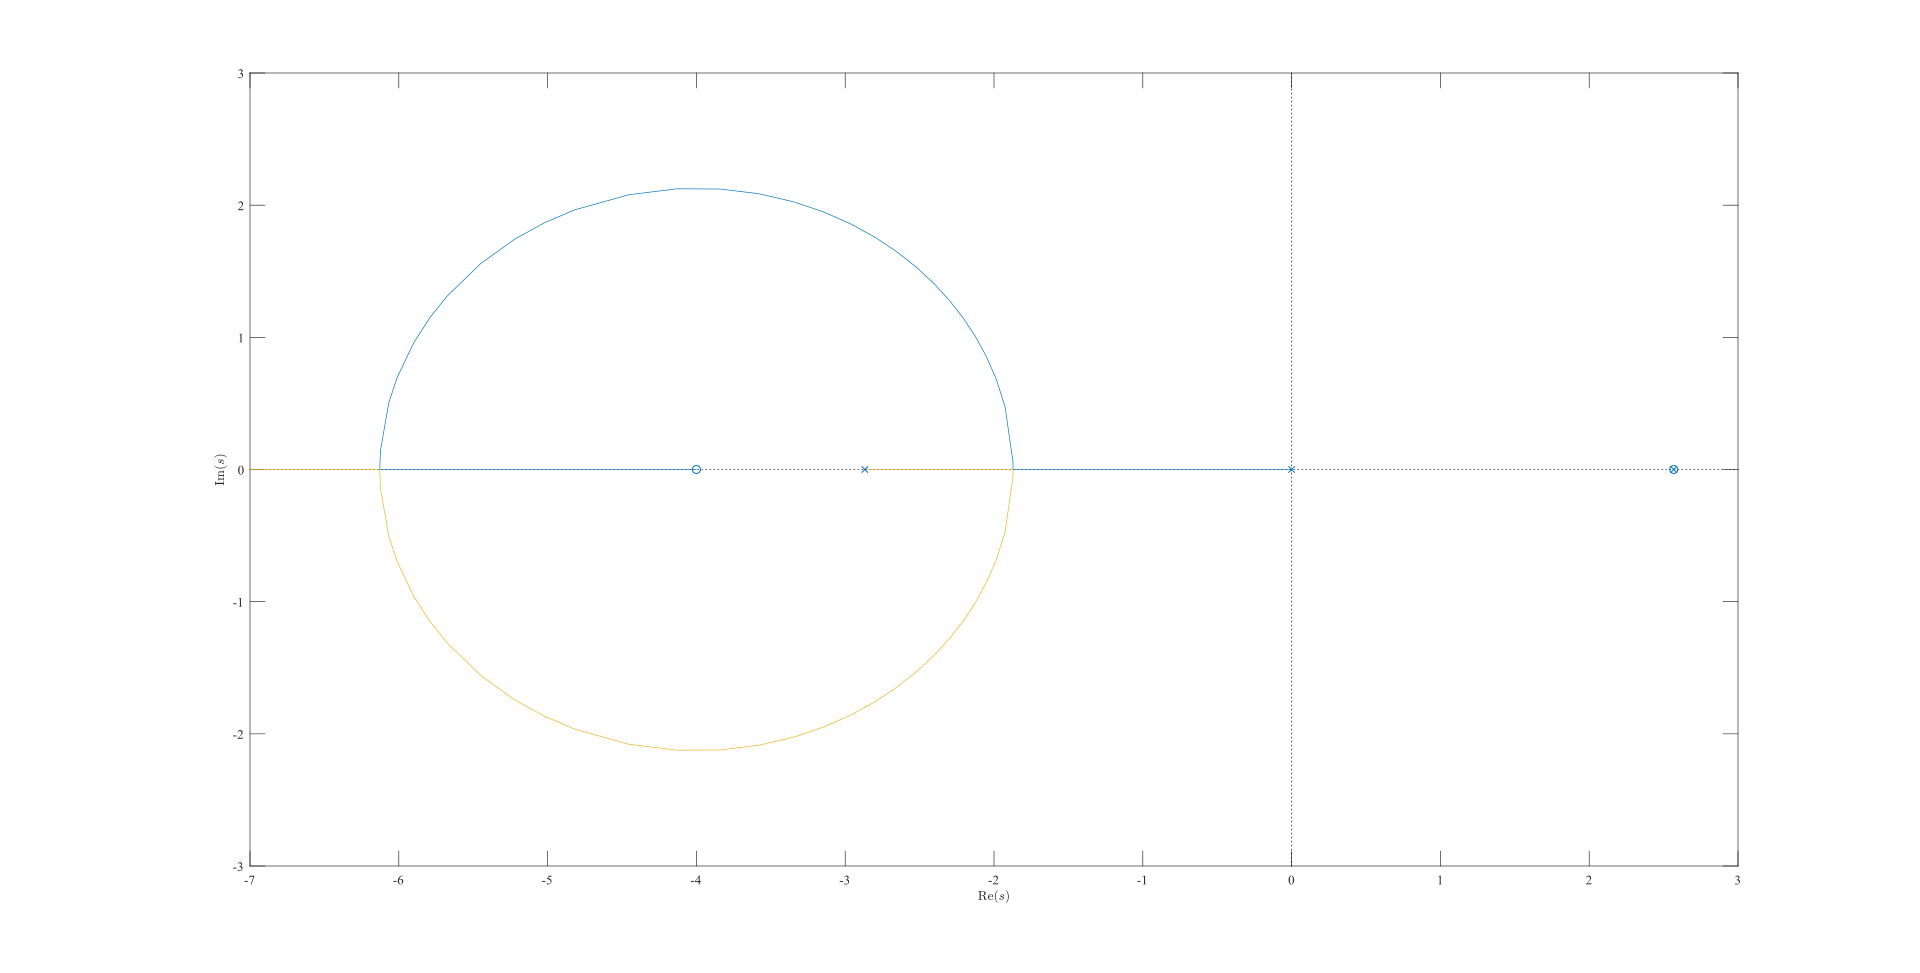
\includegraphics{images/rlocus.jpg}
  \caption{Root locus plot} \label{my_root_locus_plot}
\end{figure}
Next up is checking the performance of the entire system, see transferfunction \ref{closed_loop_system}.
\begin{equation} \label{closed_loop_system}
    T(s) = \frac{K(s) \cdot G(s)}{1+K(s)\cdot G(s)}
\end{equation}
By using the matlab function stepinfo and step, both the step responds and the information of the system can be concluded. The results with $Ti = -0.1394$, $Td = 1/1.432$ and $kp = 1.432$ gave a unstable system not worth mentioning, but by increasing the gain Kp to 2.1432 the following was observed:
\begin{itemize}
  \item RiseTime: 0.3238
  \item SettlingTime: 0.9611
  \item SettlingMin: 0.9027
  \item SettlingMax: 1.0276
  \item Overshoot: 2.7641
  \item Peak: 1.0276
\end{itemize}
\begin{figure}[htbp]
  \centering
  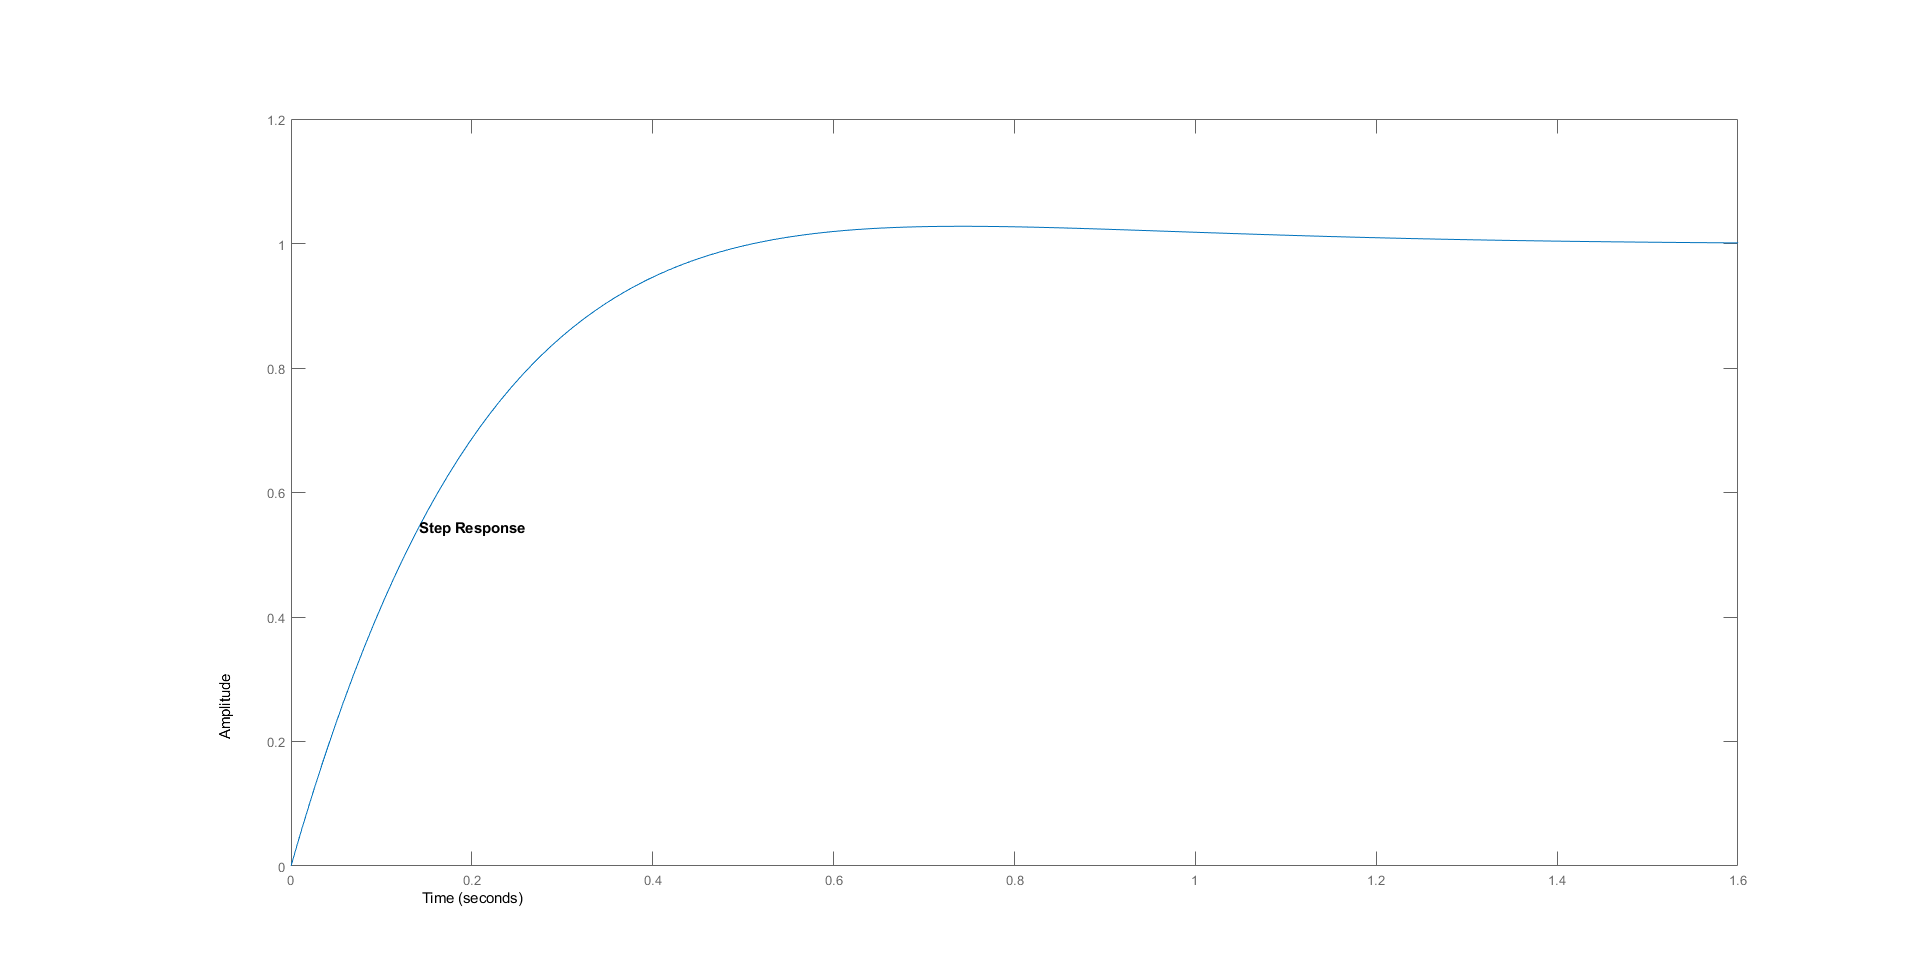
\includegraphics[width=0.7\textwidth]{images/first_kp_adjustment.jpg}
  \caption{step response for the first iteration} \label{my_first_step}
\end{figure}
Next the Kp increases to 4.132 and the following perforamnce of the system can be observed:
\begin{itemize}
  \item RiseTime: 0.1921
  \item SettlingTime: 0.6671
  \item SettlingMin: 0.9020
  \item SettlingMax: 1.0299
  \item Overshoot: 2.9873
  \item Peak: 1.0299
\end{itemize}
\begin{figure}[htbp]
  \centering
  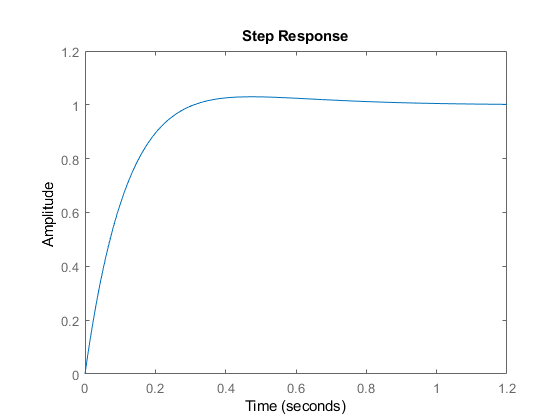
\includegraphics[width=0.7\textwidth]{images/second_kp_adjustment.jpg}
  \caption{step response for the second iteration} \label{my_second_step}
\end{figure}
The perfoamnce has technically inproved when it comes to rise time and settling time, however the desired rise time is around 1 second so it isn't an improvemnt for the desired system. The overshoot, however minute, has increased. The steady state error is eliminated as the previous with try, observed on figure \ref{my_second_step}. So this time Kp will be decreased to 2.00:
\begin{itemize}
  \item RiseTime: 0.3838
  \item SettlingTime: 1.0588
  \item SettlingMin: 0.9073
  \item SettlingMax:  1.0251
  \item Overshoot: 2.5096
  \item Peak: 1.0251
\end{itemize}
\begin{figure}[htbp]
  \centering
  \includegraphics[width=0.7\textwidth]{images/3_kp_adjustment.jpg}
  \caption{step response for the third iteration} \label{my_third_step}
\end{figure}
This time the rise time has increased and the overshoot has decreased both, however, less than desired. However the Kp can't be decreased much more before the system becomes unstable. There is also a small steady state error that can be observed on figure \ref{my_third_step}.


\subsection*{Simulation}

\begin{itemize}
  \item Simulate the linearized system with set point $\pi/3$ rad. and initial condition 0 rad.
  \item Simulate the nonlinear system model with the designed PID control.
\end{itemize}

A small report should document the above steps, with derivations, block diagrams, and graphs related
to the simulations (plot both the input and output of the system). The report must follow the provided
template.
13





\end{document}
